\documentclass[11pt,letterpaper]{article}
\usepackage[utf8]{inputenc}

%----- Configuración del estilo del documento------%
\usepackage{epsfig,graphicx}
\usepackage[left=2cm,right=2cm,top=1.8cm,bottom=2.3cm]{geometry}
\usepackage{fancyhdr}
\usepackage{lastpage}
\pagestyle{fancy}
\fancyhf{}

\usepackage{amsmath,amsthm,amssymb, tikz}
\usepackage{graphicx}
%%Use this package for matrices
\usepackage{array}
\usepackage{breqn}
\usepackage{multicol}
\usepackage{lipsum}
\usepackage{caption}
\usepackage{subcaption}
\usepackage{booktabs}

%%%%%%%%%%%%%%%%%%%%%%%%%%%%%%%%%%%%%%%%%%%%%%%%%%%%%%%%%%%%%%%%%%%%%%%%%%%%%%%%
\usepackage{amsmath}
\usepackage{amssymb}
\usepackage{graphicx}
\usepackage{subcaption}
\usepackage{mwe}
\usepackage{amsthm}
\usepackage{float}
\usepackage[export]{adjustbox}
\DeclareMathOperator*{\argmin}{argmin} 

%%%%%%%%%%%%%%%%%%%%%%%%%%%%%%%%%%%%%%%%%%%%%%%%%%%%%%%%%%%%%%%%%%%%%%%%%%%%%%%%

\usepackage{lipsum}



\begin{document}

%%%%%%%%%%%%%%%%%%%%%%%%%%%%%%%%%%%%%%%%%%%%%%%%%%%%%%%%%%%%%%%%%%%%%%%%%%%%%%%%

\begin{center}
    \begin{minipage}{10cm}
    	\begin{center}
    	\textbf{\large Project 4 Regression Analysis}\\[0.1cm]
        \textbf{Inesh Chakrabarti, Lawrence Liu, Nathan Wei}\\[0.1cm]
    	\end{center}
    \end{minipage}\hfill
\end{center}

\rule{17cm}{0.1mm}

%%%%%%%%%%%%%%%%%%%%%%%%%%%%%%%%%%%%%%%%%%%%%%%%%%%%%%%%%%%%%%%%%%%%%%%%%%%%%%%%

\section*{Introduction}
For the first part of this project we will do regression analysis. The dataset 
we chose to use is one of diamond characteristics. We will conduct regressions
to predict the price of a diamond given some features. 


\section*{Dataset}
Let us begin by understanding the dataset. The dataset consists of information
about 53940 round-cut diamonds with ten features: 
\begin{table}[ht]

\label{table1} 
\begin{tabular}{cl} 
\hline
\multicolumn{1}{c}{Feature} & \multicolumn{1}{c}{Description}\\
\hline 
    \texttt{carat} & weight of the diamond (0.2–5.01) \\
    \texttt{cut} & quality of the cut (Fair, Good, Very Good, Premium, Ideal) \\
    \texttt{color} & diamond colour, from J (worst) to D (best) \\
    \texttt{clarity} & a measurement of how clear the diamond is (I1 (worst),  
    SI2, SI1, VS2, VS1, VVS2, VVS1, IF (best)) \\
    \texttt{x} & length in mm (0–10.74) \\
    \texttt{y} & width in mm (0–58.9) \\
    \texttt{z} & depth in mm (0–31.8) \\
    \texttt{depth} & total depth percentage \\
    \texttt{table} & width of top of diamond relative to widest point (43-95) \\
    \texttt{price} & price in US dollars (\$326-\$18,823)
\end{tabular}
\end{table}


%%%%%%%%%%%%%%%%%%%%%%%%%%%%%%%%%%%%%%%%%%%%%%%%%%%%%%%%%%%%%%%%%%%%%%%%%%%%%%%%

\subsubsection*{Question 1.1}
\begin{figure}[H]
    \centering
   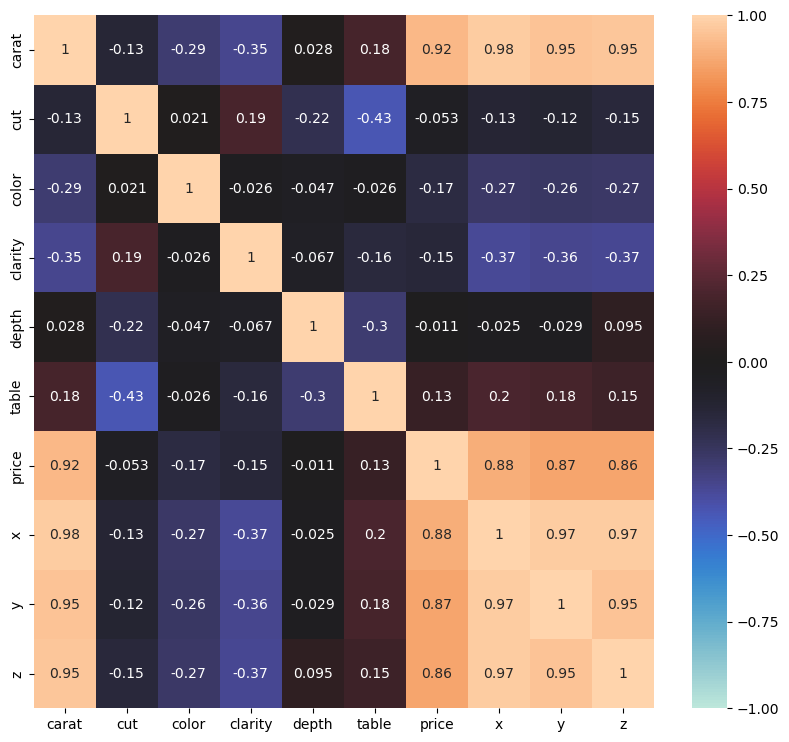
\includegraphics[width=0.5\linewidth]{../Figures/Question-1/datasetCorrHeatmap.png}
   \caption{Feature Pearson Correlation Heatmap}
   \label{fig:corr_hm}
\end{figure}

We will be using the nine features to predict the \texttt{price}. We can begin by 
computing the Pearson correlation matrix heatmap for these features in 
the dataset in Figure 1. Note that a pearson correlation coefficient $r$ is 
defined as such:
\begin{equation}
r=\dfrac{\sum_i \left(x_i-\bar{x}\right)\left(y_i-\bar{y}\right)}{\sqrt{
\sum_i\left(x_i-\bar{x}\right)^2\sum_i\left(y_i-\bar{y}\right)^2
}}
\end{equation}
We have assigned quantitative values to
the qualitative labels \texttt{cut},\texttt{color},\texttt{clarity} as ascending 
natural numbers based on ideality.

\begin{table}[H]
    \begin{subtable}[H]{0.45\textwidth}
        \centering
        \begin{tabular}{c l}
            \hline
            Feature & \multicolumn{1}{c}{Correlation}         \\
            \hline 
        \texttt{carat}   & 0.9215914337868304    \\
        \texttt{cut}     & -0.05349263851362828  \\
        \texttt{color}   & -0.1725093772499559   \\
        \texttt{clarity} & -0.14680175361025616  \\
        \texttt{depth}   & -0.010647725608533299 \\
        \texttt{table}   & 0.12713358133531918   \\
        \texttt{x}       & 0.8844357793744166    \\
        \texttt{y}       & 0.865421694764742     \\
        \texttt{z}       & 0.861250266123968    
        \end{tabular}
        \caption{Price}
        \end{subtable}
        \begin{subtable}[H]{0.45\textwidth}
            \centering
            \begin{tabular}{c l}
                \hline
                Feature & \multicolumn{1}{c}{Correlation}         \\
                \hline 
            \texttt{carat}   & 0.7694571626172851    \\
            \texttt{cut}     & 0.00542011950342582   \\
            \texttt{color}   & -0.011980043670033661 \\
            \texttt{clarity} & 0.04512538515850012   \\
            \texttt{depth}   & -0.03572374489729493  \\
            \texttt{table}   & 0.08458507638109278   \\
            \texttt{x}       & 0.7873455524189906    \\
            \texttt{y}       & 0.7717301198408058    \\
            \texttt{z}       & 0.7655421629234554   
            \end{tabular}
            \caption{Price per Carart}
        \end{subtable}
        \caption{Pearson Correlation Coefficients}
    \end{table}

The values for correlation for \texttt{price} is given in 
Table 1(a). We see that, unsurprisingly, there is a massive collection of high 
correlation squares at the bottom right. These indicate high Pearson 
correlation coefficient between \texttt{price} and \texttt{x}, \texttt{y}, 
\texttt{z}. Similarily, there is also a high correlation with \texttt{carat}.
All of these suggest that the size of the diamond itself is the most significant 
predictor as to its price. \\ 

However, unexpectadly, we had a negative perason coeffciient for the quality of 
the \texttt{cut}, \texttt{color}, and \texttt{clarity}. This was odd, so we
similarily calculated the Pearson correlation values for Price per Carat instead, 
given in Table 1(b). We observed that the coefficient for \texttt{cut} and 
\texttt{clarity} became slightly positive, while color became close to zero. 
These seemed more in line with our expectations,and confirmed that the rarity of 
high carat and high clarity in a diamond at the same time was making the 
corresponding values in Table 1(a) negative. 

\subsubsection*{Question 1.2}
\begin{table}[H]
    \begin{subtable}[H]{0.45\textwidth}
    \centering
    \begin{tabular}{c l}
        \hline
        Feature & \multicolumn{1}{c}{Skewness} \\
        \hline
        \texttt{carat} & 1.116645920812613  \\ \
        \texttt{depth} & -0.08229402630189467 \\ \
        \texttt{table} &  0.7968958486695427\\ \
        \texttt{x} & 0.3786763426463927  \\ \
       \texttt{y} & 2.4341667164885554  \\ \
        \texttt{z} & 1.5224225590685583  \\ \
    \end{tabular}
    \caption{Before Processing}
    \end{subtable}
    \begin{subtable}[H]{0.45\textwidth}
        \centering
        \begin{tabular}{c c l}
            \hline
            Feature & Method & \multicolumn{1}{c}{Skewness} \\
            \hline
            \texttt{carat} & Box Cox & 0.020450070764268666 \\ \
            \texttt{depth} & No Change & -0.08229402630189467 \\ \
            \texttt{table} &  Logrithm & 0.5993289324435086\\ \
            \texttt{x} & No Change & 0.3786763426463927  \\ \
            \texttt{z} & Square Root & 0.0139742634447758  \\ \
        \end{tabular}
        \caption{After Processing}
        \end{subtable}
    \caption{Skewness of Features}
\end{table}

\begin{figure}[H]
    \centering
    \begin{subfigure}[b]{0.45\textwidth}
        \centering
        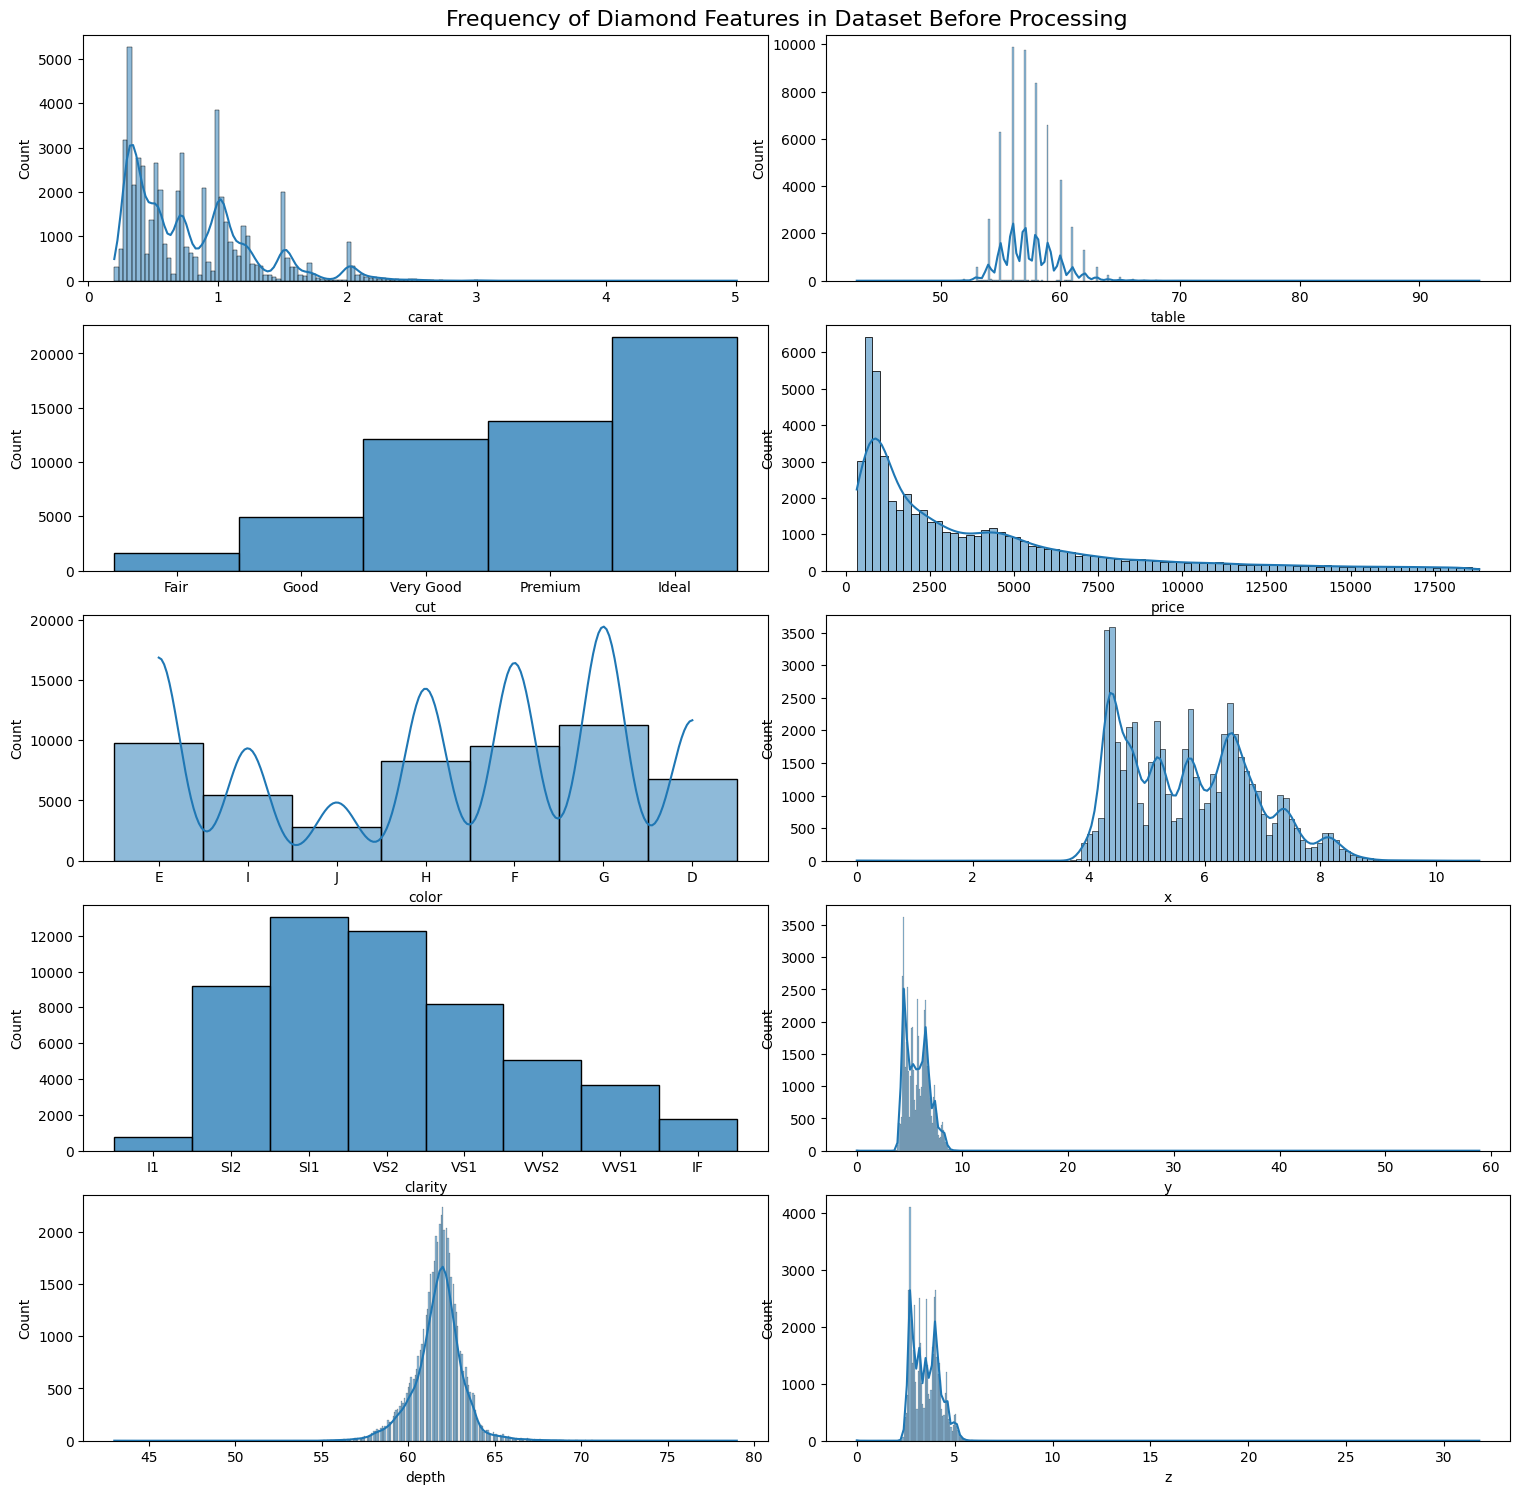
\includegraphics[width=\textwidth]{../Figures/Question-1/featureprehist.png}
        \caption{Before Processing}
        \label{fig:clarityBox}
    \end{subfigure}
    \hfill
    \begin{subfigure}[b]{0.45\textwidth}
        \centering
        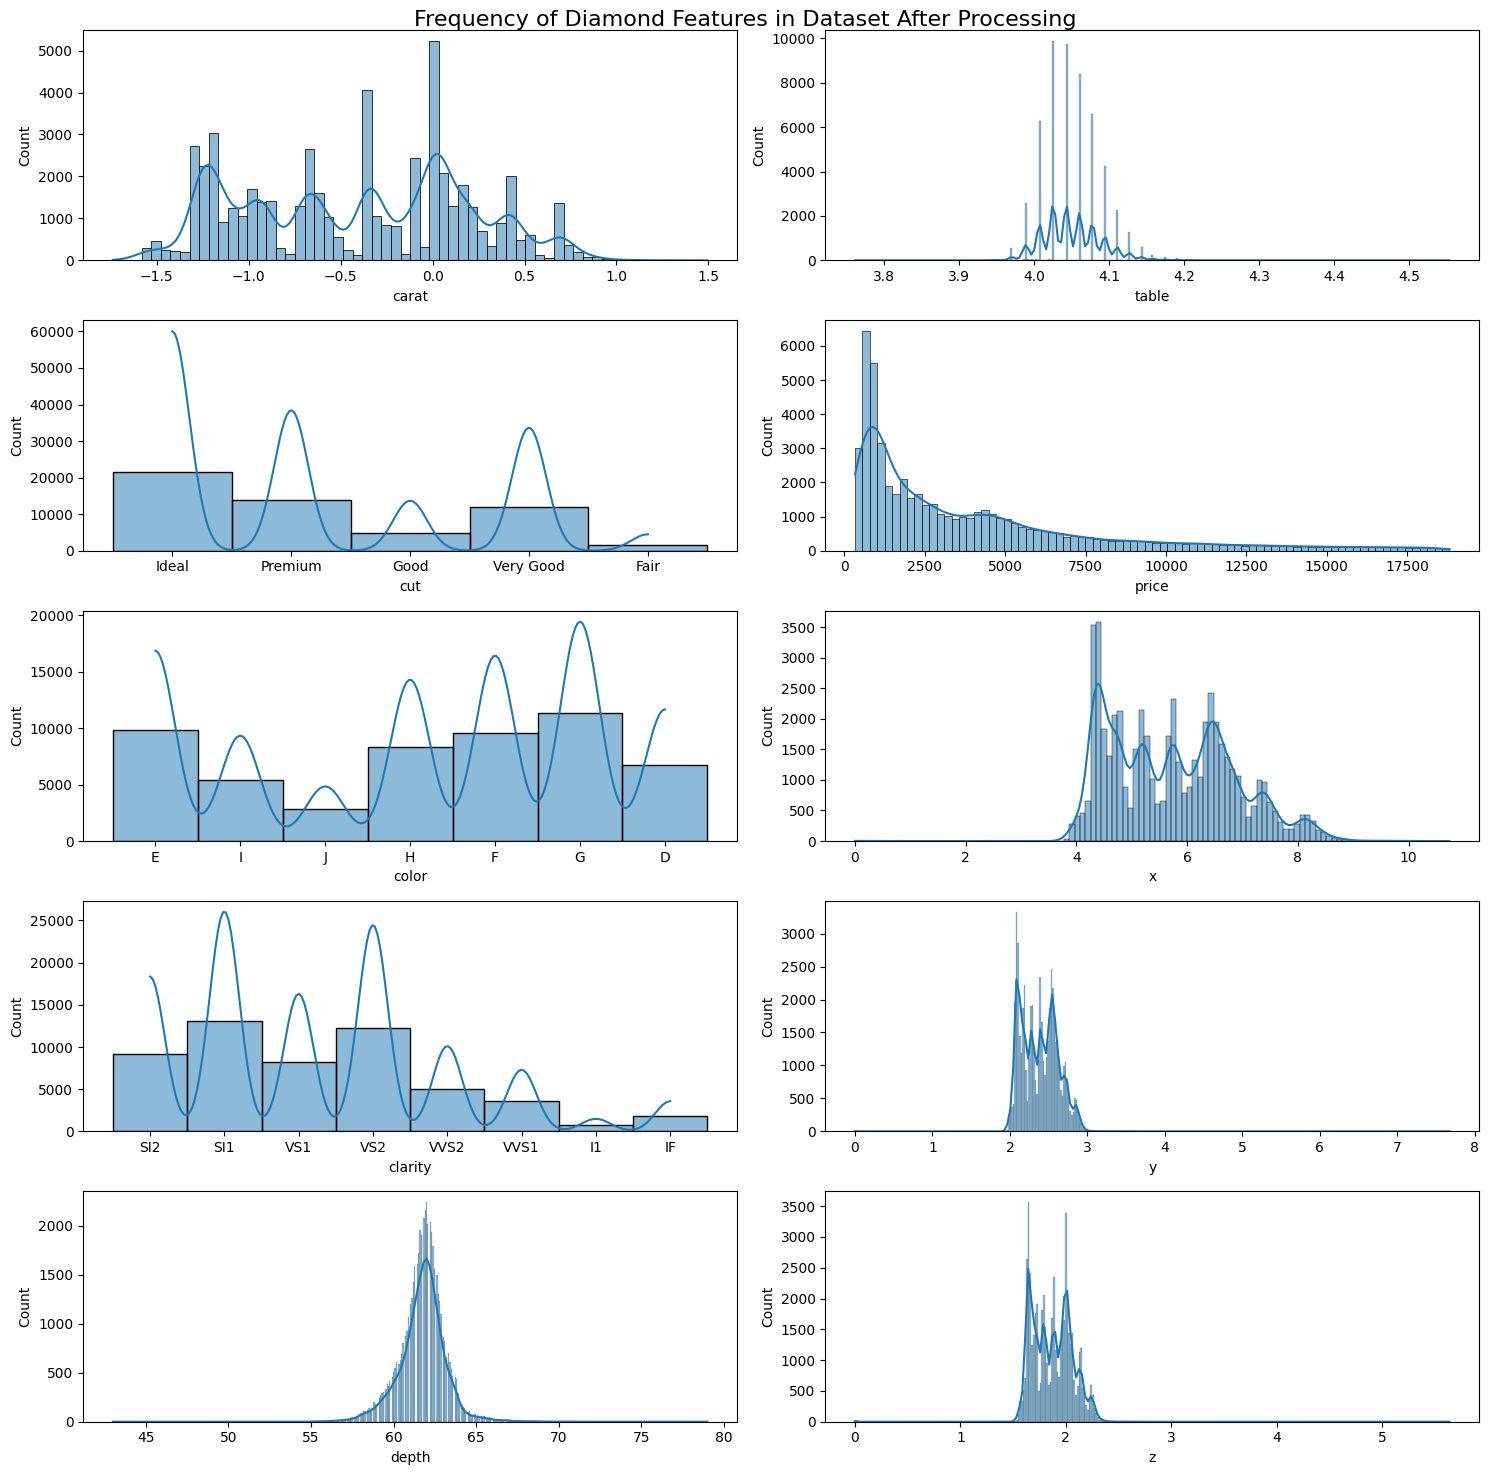
\includegraphics[width=\textwidth]{../Figures/Question-1/featureposthist.png}
        \caption{After Processing}
        \label{fig:colorBox}
    \end{subfigure}
       \caption{Histogram and KDE for Features}
       \label{fig:boxPlots}
\end{figure}

%%%%%%%%%%%%%%%%%%%%%%%%%%%%%%%%%%%%%%%%%%%%%%%%%%%%%%%%%%%%%%%%%%%%%%%%%%%%%%%%
Now, we examine the frequency distributions within each feature. We find that 
some of our numerical features are somewhat skewed—apparent from Table 2(a) and
Figure 2(a). We target a skewness less than $0.5$, as this would imply that the 
distribution is somewhat symetric. As such, we try three different methods: 
square-root, logrithm, and box-cox transformation. The first two are somewhat
self-explanatory; box-cox uses a non-zero value of $\lambda$ and conducts the
following transformation:
\begin{equation}
y_{\lambda}^{'} = \dfrac{y^{\lambda}-1}{\lambda \cdot \bar{g}_y^{\lambda-1}}
\end{equation}
where $\bar{g}_y$ is defined as the geometric mean of $y$. \\
We next try all of these methods, along with no transformatino, and take the 
minimum to try to minimize skewness in our data. The results are shown in Table 
2(b) and Figure 2(b).


\subsubsection*{Question 1.3}

\begin{figure}[H]
    \centering
    \begin{subfigure}[b]{0.3\textwidth}
        \centering
        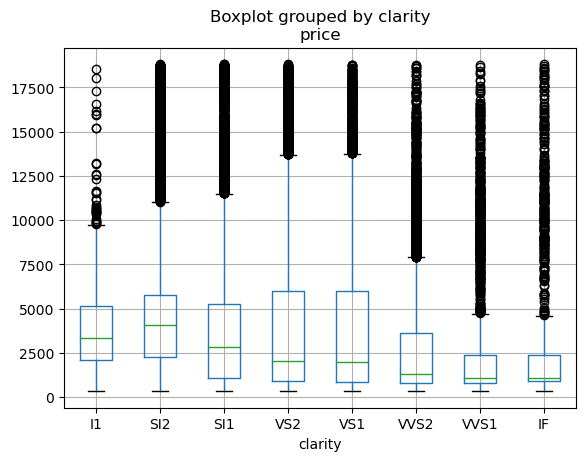
\includegraphics[width=\textwidth]{../Figures/Question-1/clarityBox.png}
        \caption{Clarity}
        \label{fig:clarityBox}
    \end{subfigure}
    \hfill
    \begin{subfigure}[b]{0.3\textwidth}
        \centering
        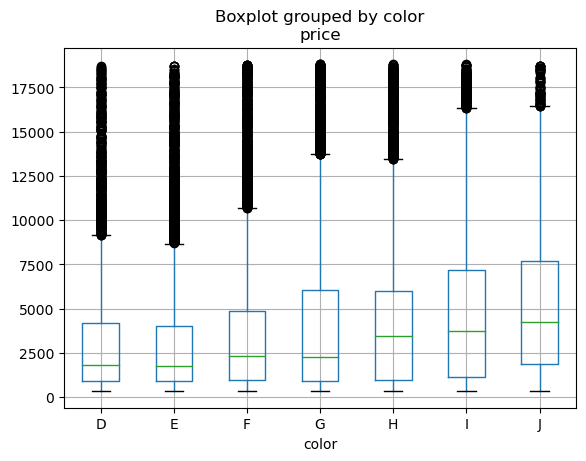
\includegraphics[width=\textwidth]{../Figures/Question-1/colorBox.png}
        \caption{Color}
        \label{fig:colorBox}
    \end{subfigure}
    \hfill
    \begin{subfigure}[b]{0.3\textwidth}
        \centering
        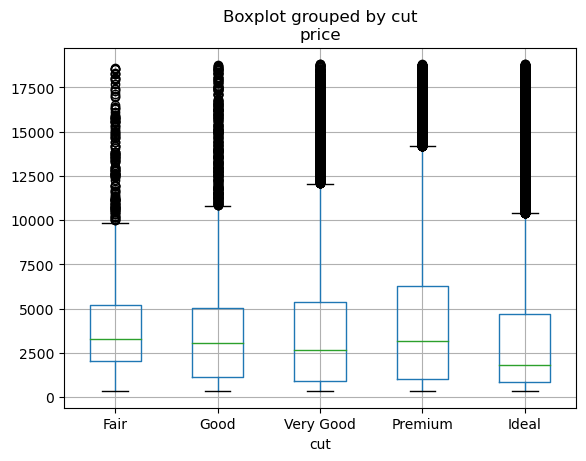
\includegraphics[width=\textwidth]{../Figures/Question-1/cutBox.png}
        \caption{Cut}
        \label{fig:cutBox}
    \end{subfigure}
       \caption{Categorical feature vs price boxplots}
       \label{fig:boxPlots}
\end{figure}

Begin by noting that in these boxplots, the features are arranged from left to right
in terms of ascending desirablity. \\\\
Begin by observing the boxplot for \texttt{clarity}. Note that the trend for the outlier cutoffs
$(1.5\times \text{IQR})$ seems to mirror the frequency histogram plot in Figure 2(a). This
is somewhat interesting, as this implies that we simply find more expensive diamonds 
of average clarity, which also have a wider range of prices. Meanwhile, the 
diamonds with the best clarity seem to have a low cutoff, which could be attributed to
the small sample size, but also the fact that these diamonds are also likely to be smaller. 
This is apparent from Figure 1, where we see that there is a negative coefficient in the case
comparing \texttt{clarity} with \texttt{x}, \texttt{y}, and \texttt{z}.
Note that size of the diamond was established as the best predictor for the price of the diamond 
from earlier. Meanwhile, it is apparent that the diamond with worst clarity have few that
breach the 10000 dollar price mark, as we only see a few individual dots on the boxplot indicating
these diamonds. \\\\
Now, let us analyze the boxplot for \texttt{color}. We see that there is a negative trend 
for the outlier cutoff as the desirability of the color increases. This 
To analyze the boxplot for \texttt{cut}, we need to also look as the histogram 
of diamond features in Figure 2(a). Note that we also have increasing numbers of 
diamonds as we move left to right. We see that the data generally follows our expectation,
as the outlier cutoff seems to be higher for each one. However, 
this changes when the \texttt{cut} is Ideal. This makes sense, most of the diamonds are
cut ideally, and smaller diamonds are also probably easier to cut well; meanwhile, 
if a diamond isn't cut very well, but there was some attempt to cut it to some reasonable
extent, it was probably very large. This explains why Ideal seems to break the 
observed trend. \\\\
Finally, let us observe the boxplot for \texttt{cut}. This plot can be explained with 
similar explanation to that of \texttt{clarity}. In fact, 


\subsubsection*{Question 2.1}
Now, before we train our regression models, we begin by splitting our data into 
training and testing sets. As such, we must now standardize the feature columns.
The function used to do this, \texttt{scaledTrainTest()}, as well as \texttt{
scaledTrainTestSplit()} can be found in \texttt{utils.py}.

\subsubsection*{Question 2.2}
Next, we begin with feature selection. We note that some of the features may not
be useful or may cause overfitting in our models as they do not carry useful 
useful information about the variable that we are trying to predict. To tell 
whether this is the case, we use two metrics: Mutual Information (MI) and F 
score.

\begin{figure}[H]
    \centering
   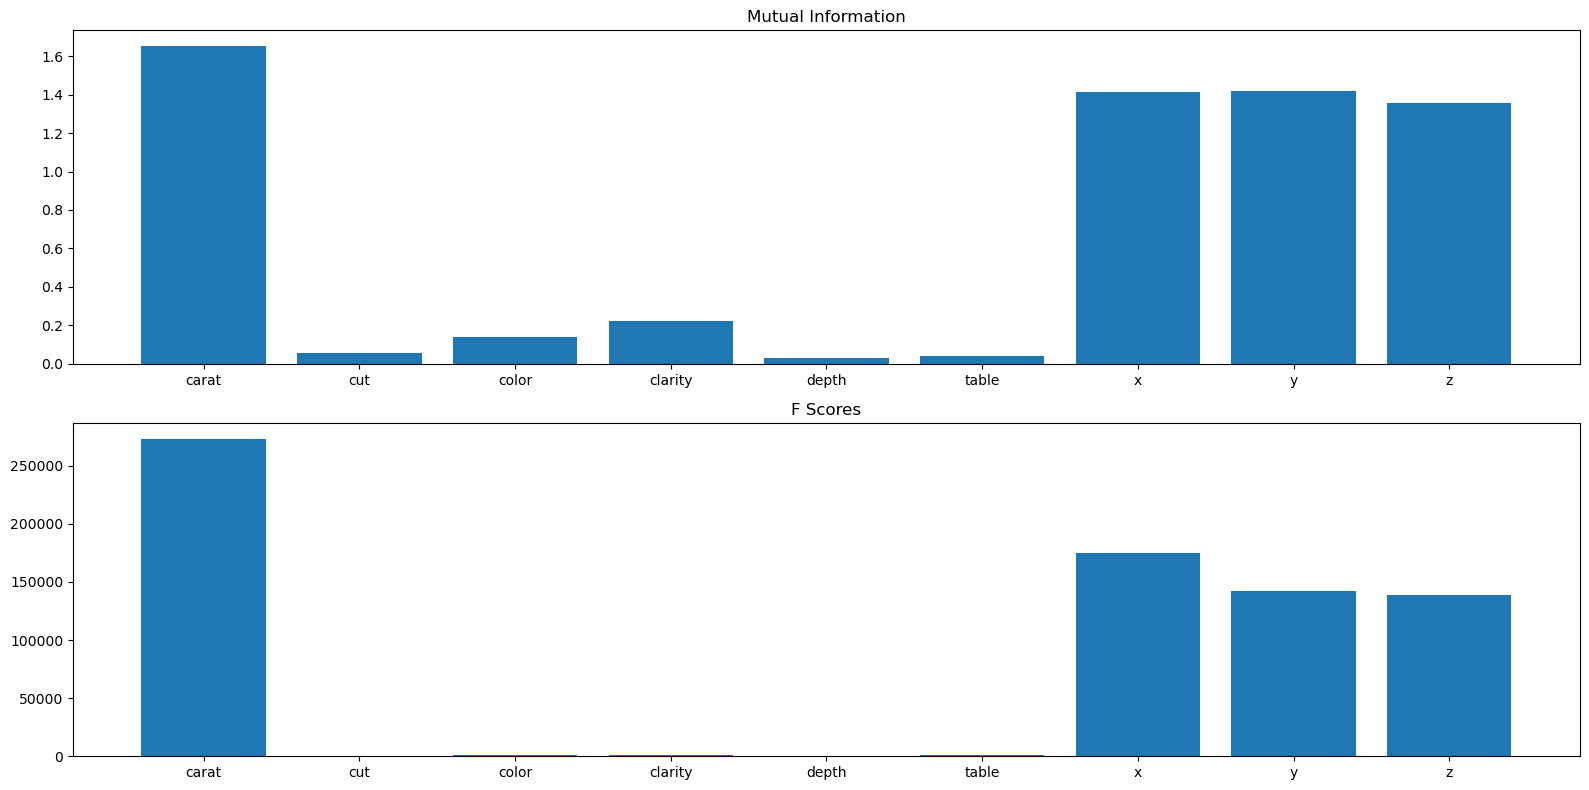
\includegraphics[width=0.8\linewidth]{../Figures/Question2/mi.png}
   \caption{Bar graph of F score and Mutual Information for features}
\end{figure}
\begin{table}[!ht]
    \centering
    \begin{tabular}{c l l}
    \hline
        Feature & Mutual Information & F Score \\ \hline
        \texttt{carat} & 1.64589286853222835 & 273144 \\ \
        \texttt{cut} &0.058351547792578895 & 139 \\ \
        \texttt{color} &0.13968295427702282 & 1465 \\ \
        \texttt{clarity} & 0.21672877051000627 & 1079 \\ \
        \texttt{depth} & 0.030486803506200033 & 5.074 \\ \
        \texttt{table} & 0.03818752327438668 & 802 \\ \
        \texttt{x} & 1.4058664238563194 & 174973 \\ \
       \texttt{y} & 1.4172107199595354 & 142130 \\ \
        \texttt{z} & 1.3569258463570115 & 138947 \\ \
    \end{tabular}
    \caption{Mutual Information and F Score Values for features}
\end{table}
It is clear by observation from Figure 3 and Table 2 that the lowest mutual 
information is present in \texttt{depth} and \texttt{table}. It is also 
important to note that the mutual information in \texttt{cut} is also very small. 
This makes sense as we saw earlier that the Pearson correlation coefficient for 
\texttt{cut} with respect to price per carat was almost zero. Similarily, the 
Pearson correlation coefficients for depth and table were very close to zero. \\ 

From this point, we will be testing the regression models without these three 
features, and with these three features and comparing the performance to 
determine the general performance.

\section*{Regression Models}
\subsubsection*{Question 3}
%%%%%%%%%%%%%%%%%%%%%%%%%%%%%%%%%%%%%%%%%%%%%%%%%%%%%%%%%%%%%%%%%%%%%%%%%%%%%%%%
For this entire section we perform 10-fold cross validation and then measure
the average RSME error for the training and validation sets. For the random 
forest model we also measure "Out-of-Bag Error" and $R^2$ score. \\
To explain OOB error, let us first examine how a Random Forest algorithm with
bootstrapping works. If we bootstrap, we sample the training data, and then use 
this small sample of the training data in order to train a single decision tree model.
We can then ensemble many such trees, all trained with different samples of the original
data. OOB error is calculated on the training set, where we calculate the average error 
of the trees' predictions on data that was not included in its bootstrap sample. \\\\
$R^2$ score is normally used as the coefficient of determination—that is—the proportion
of the variation in the labels that can be predicted from the features. For random 
forests, we compute it as:
\[R^2 = 1- \dfrac{\text{MSE}}{\text{Var}(\text{labels})}
    \]
Note that $R^2$ for non-linear predictors like random forest can in fact be negative.

\subsection*{Linear Regression}
\subsubsection*{Question 4.1}
We begin with a simple regression, least square linear regression. Begin by 
noting the optimization problem:
\begin{equation}
    \argmin_{\theta} \dfrac{1}{2}||\textbf{Y}-\theta^T\hat{\textbf{X}}||^2
\end{equation}
Taking the derivative with respect to $\theta$ and setting it equal to zero 
gives us 
\begin{equation}
\theta = \left(\textbf{X}^T\textbf{X}\right)^{-1}\textbf{X}^T\textbf{Y}
\end{equation}
Now, we can add regularization terms, beginning with the simple L1 
regularization, also known in this case as a Lasso regression. This would make 
our new optimization problem:
\begin{equation}
    \argmin_{\theta} \dfrac{1}{2}||\textbf{Y}-\theta^T\hat{\textbf{X}}||^2 + 
    \alpha ||\theta||
\end{equation}
Note that in this case, our learned values for $\theta$ would become somewhat 
sparse as L1 regularization linearly penalizes any non-zero parameters.
As such, the gradient for the regularization term does not change until the 
parameter is zero, which leads to sparsity. However, in this case, as there 
aren't many terms, we would simple disconsider features that aren't very 
important. \\ \\
With L2 regularization, also known as a Ridge regression, we would have:
\begin{equation}
    \argmin_{\theta} \dfrac{1}{2}||\textbf{Y}-\theta^T\hat{\textbf{X}}||^2 + 
    \lambda ||\theta||^2
\end{equation}
Note in this case, we wouldn't have parameters that are zero; rather, we would 
have extremely small parameters. This is because the gradient for L2 
regularization decreases rapidly as the parameter itself becomes smaller and 
smaller due to the parabolic nature of the term. 

\subsubsection*{Question 4.2 and 4.3}


\begin{table}[H]
    \centering
    \begin{tabular}{clll}
        \hline
    Model & \multicolumn{1}{c}{Description} & \multicolumn{1}{c}{Train RSME} & \multicolumn{1}{c}{Test RSME} \\
    \hline
    \texttt{1}     & Features processed              & 1434.7215231192772                                                     & 1443.41152861054185                                                      \\
    \texttt{2}     & Features unprocessed            & 1216.495767837737                                                       & 1217.7987618616985                                                      \\
    \texttt{3}     & Features processed using $log$(\texttt{price})   & 963.6508209107394                                                      & 963.0840609301274                                                       \\
    \texttt{4}     & Features unprocessed using $log$(\texttt{price}) & 1215.167267164955                                                      & 1292.934288205552                                                      
    \end{tabular}
    \caption{Ordinary Least Squares Regression Model}
    \end{table}

Beginning with ordinary least squares regression, I first varied the 
number of features available to the model based on mutual information and quickly 
found that keeping all the features led to the best regression model. This makes 
sense due to the nation of a linear regression—if a feature isn't very relevant, 
its associated parameter will be very small—and so for Ridge and Lasso, we also
kept all of the features. \\\\
\begin{figure}[H]
    \centering
    \begin{subfigure}[b]{0.475\textwidth}
        \centering
        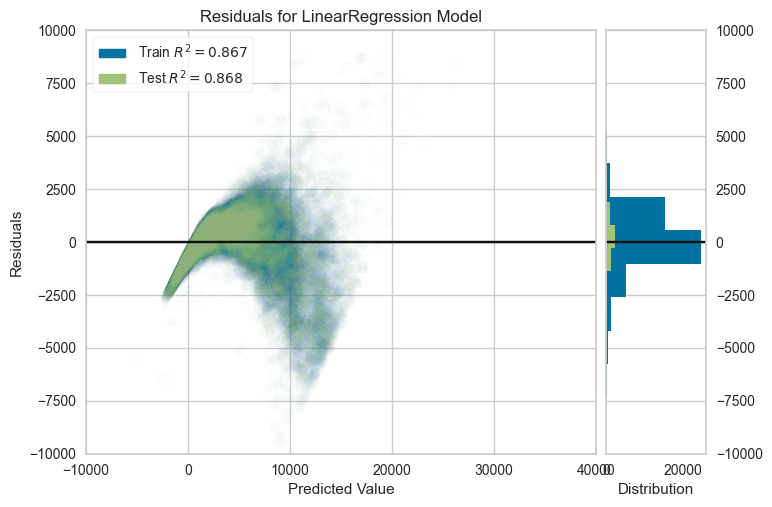
\includegraphics[width=\textwidth]{../Figures/question4/linresplot1.png}
        \caption[Network2]%
        {{Model \texttt{1} Residuals }}    
    \end{subfigure}
    \hfill
    \begin{subfigure}[b]{0.475\textwidth}  
        \centering 
        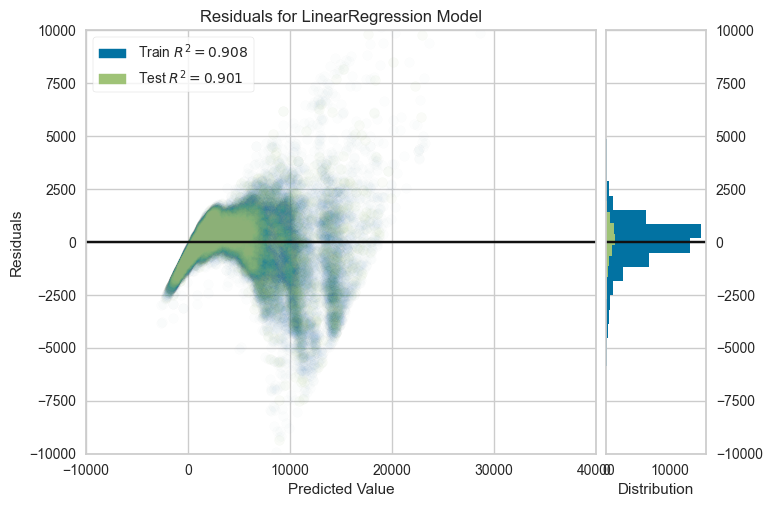
\includegraphics[width=\textwidth]{../Figures/question4/linresplot2.png}
        \caption[]%
        {Model \texttt{2} Residuals}    
    \end{subfigure}
    \vskip\baselineskip
    \begin{subfigure}[b]{0.475\textwidth}   
        \centering 
        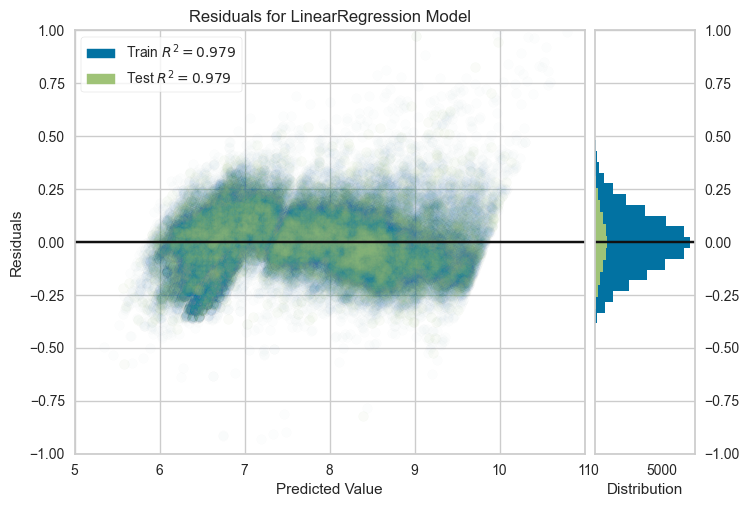
\includegraphics[width=\textwidth]{../Figures/question4/linresplot3.png}
        \caption[]%
        {{Model \texttt{3} $log$ Residual}}    
    \end{subfigure}
    \hfill
    \begin{subfigure}[b]{0.475\textwidth}   
        \centering 
        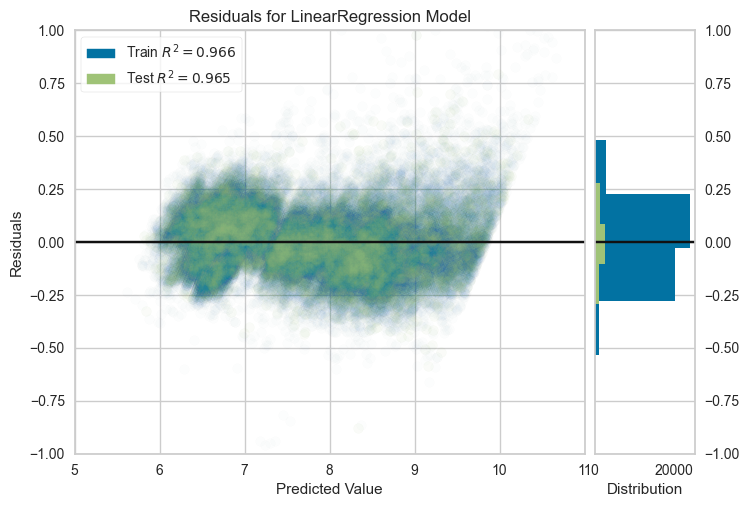
\includegraphics[width=\textwidth]{../Figures/question4/linresplot4.png}
        \caption[]%
        {{Model \texttt{4} $log$ Residuals}}    
    \end{subfigure}
    \caption{Residual Plots} 
\end{figure}
We then tested the linear regression model with processed data (deskewed as in 
Question 1.2) and unprocessed data. We noted that the model without processed features
seemed to perform much better as shown in Table 4 and visualized in Figure 5. Note that
Model \texttt{2}'s residual histogram is distributed far more sysmtetrically than 
Model \texttt{1}, implying that the linear regression fit better in this case.
However, we see in both Figures 5(a) and 5(b) that Models \texttt{1} and \texttt{2} 
predict many of the prices to be negative. \\\\
As such, we decided to test the model by taking the natural logrithm of 
\texttt{price} before fitting the regression. Note in Table 4 that with unprocessed 
Features, this model performed about the same, but with processed features the RSME 
decreased very significantly. We also see that our new $log$ residual plots seem to 
follow a linear trend, which makes sense as this implies that the error is increasing
as the price of the diamond itself increases. We also note that unlike earlier, Model
\texttt{3} has normally distributed residuals while Model \texttt{4} does not. This is
interesting, because this is the opposite of Models \texttt{1} and \texttt{2}; that is,
this time, the model with deskewed data has the more normal distribution of residuals.\\\\

Next, we test the Lasso Model by iterating through alpha values $10^k$ such that 
$k\in \mathbb{Z}$ and $-4 \geq k \leq 1$. We also try both the $log$(\texttt{price})
model, and try both with and without deskewing. As seen in Table 5, we see that the best performming 
model is the same as for ordinary least squares regression, as well as the general trends across 
the models. The only difference in this case that we see is that leaving the features unprocessed 
while also taking the $log(\texttt{price})$ leads to the error blowing up. We note that this issue 
persists for all future models referred to in this report as well. 

\begin{table}[H]
    \centering
    \begin{tabular}{clcll}
        \hline
    Model & \multicolumn{1}{c}{Description} & \multicolumn{1}{c}{Best Alpha} & \multicolumn{1}{c}{Best Train RSME} & \multicolumn{1}{c}{Best Test RSME} \\
    \hline
    \texttt{1}     & Features processed       & 1       & 1434.8446180295655                                                     & 1443.270394653097                                                      \\
    \texttt{2}     & Features unprocessed    & 1        & 1216.5716991188874                                                      & 1217.1322328759766
    \\
    \texttt{3}     & Features processed using $log$(\texttt{price})  & 0.001 & 953.1890102312589                                                     & 952.4417958988445                                                       \\
    \texttt{4}     & Features unprocessed using $log$(\texttt{price}) & 10 &  4270.277347211739                                                   & 4270.276711329372                                                   
    \end{tabular}
    \caption{Lasso Regression Model}
\end{table}

Next we test the Ridge model with all the same parameters are the Lasso model, except
we also test whether or not feature standardization is palying a role in improving 
the model performance. Note the description column has been left out as it is the same as the previous 
two models. We see in Table 6 that contrary to our expectations, scaling/standardizing the features did not 
seem to play a very big roll in improving the model. This was surprising, given how a linear regression is 
usually sensitive to changes in magnitude (making scaling beneficial). 

\begin{table}[H]
    \centering
    \begin{tabular}{cccll}
        \hline
    Model & Standardized &Best Alpha & \multicolumn{1}{c}{Best Train RSME} & \multicolumn{1}{c}{Best Test RSME} \\
    \hline
    \texttt{1}   & Yes      & 10       & 1434.8513489310335                                                   &  1442.9008267138393                                                    \\
    \texttt{1}   & No        & 10       & 1435.8556914721148                                                  & 1442.1066793353307                                                  \\
    \texttt{2}   & Yes        & 10      & 1216.6969576343665                                                   & 1217.9346926613257                                                     \\
    \texttt{2}   & No        & 1      & 1216.4978665798574                                               & 1217.7934651327528                                                   \\
    \texttt{3}   & Yes        & 0.001       & 964.0857752044615                                                    &  963.5016367407248                                                    \\
    \texttt{3}   & No       & 0.0001       & 963.4272568650325                                                   &962.8249050664665                                                     \\
    \texttt{4}   & Yes        & 1       & 1215.16766015031                                                   & 56321.703744924875                                                     \\
    \texttt{4}   & No       & 1       & 1215.1676667481079                                                  & 56321.78526878937                                                    
    \end{tabular}
    \caption{Ridge Regression Model}
\end{table}

Ultimately, we find that our best performing model was Lasso Model \texttt{3} with an alpha value of 
0.001, as this gave us the lowest RSME of all our linear regression models.


\subsubsection*{Question 4.4}
$p$-values for different features tell us the chance that a certain parameter is zero—
that is, a parameter corresponding to a certain feature is zero. This means that if a
p-value for a feature is very small, the feature is also probably not very important to
the linear model. In other words, the features with the smallest $p$-values would be the
most significant features. 


\subsection*{Polynomial Regression}

\subsubsection*{Question 5.1}

\begin{table}[ht]
\centering
    \label{table1} 
    \begin{tabular}{cl} 
    \hline
    \multicolumn{1}{c}{Feature} & \multicolumn{1}{c}{Mutual Information}\\
    \hline 
        $\texttt{carat} \times \texttt{clarity}$ & 1.8159676557242 \\
        $\texttt{carat} \times \texttt{clarity}^2$& 1.8052014657565039 \\
        $\texttt{carat} \times \texttt{color}^2$ & 1.7327044648084868 \\
        $\texttt{carat} \times \texttt{clarity}^4$ & 1.7102713903040332 \\
        $\texttt{carat} \times \texttt{color}^2 \texttt{clarity}^2$ & 1.6728060460257277 
    \end{tabular}
    \caption{Most Salient Polynomial Features}
    \end{table}
After creating an array of the polynomial features, we find, unsurprisingly, that \texttt{carat} is involved in all 
of them. However, we never use a higher power of \texttt{carat}—rather, we multiply by different powers of 
\texttt{clarity}, and in one case by $\texttt{color}^2$. This is interesting, as earlier it seemed as if all of the 
cateogrical features were either not very important, or we made some mistake in assigning ascending natural numbers 
as values for them. However, we see here that the product is somewhat valuable. This confirms our findings 
when we analyzed Figure 3 in Question 1.3; we find that keeping \texttt{carat} constant, 
higher values for \texttt{clarity} and \texttt{color} do in fact increase the price of the diamond. This confirms 
that the misleading trends were simply due to the rarity of larger diamonds as we have better \texttt{clarity} and 
\texttt{color}. Thus, although \texttt{caraat} is by far the most important singular feature, we find that when used 
in conjunction, \texttt{clarity} and \texttt{color} can be interprretted to have some meaning as well. \\\\

Interestingly, features like \texttt{x}, \texttt{y}, and \texttt{z} that had high mutual information 
were not included in the most salient feature terms. I concluded that this was because 
the information from \texttt{x}, \texttt{y}, and \texttt{z} is encompassed within 
\texttt{carat} and the singular dimension doesn't tell us as much about the diamond 
as the weight. 


\subsubsection*{Question 5.2}
In order to test and find the best polynomial degreee, we tested integer values between 2 and 6 inclusive while 
also testing different alpha values between $10^{-3}$ and $10^2$ for the Ridge regularization. We quickly notice that the higher degree polynomials 
are almost definitely overfitting, with extremely low training error and extremely high validation error.
This makes sense, as higher order polynomials are less generalized in shape, and tend to try to fit the data 
more "perfectly"—in other words, it's simply a more complicated model. We see that the model is performing much better than 
the linear regression almost universally, as the best linear model, which involved taking the logrithm of \texttt{price} 
is still worse than the best polynonimal model. Note that the best polynomial model was of 5th degree. Similarily note that 
our alpha constant values are very high, meaning that we've had to add extremely high amounts of regularization to our model because of the
overfitting nature of polynomial regression. Note that the non-linear models so far have performed best—including the  $log(\texttt{price})$ 
linear regression and now the polynomial regression. 

\begin{table}[H]
    \centering
        \label{table1} 
        \begin{tabular}{cccll} 
        \hline
        Degree & log vs raw Price & Best Alpha & Training RMSE & Testing RMSE \\
        \hline 
        2 & Raw & 10 & 900.3779319488907 & 932.1444972450224 \\
        3 & Raw & 10& 877.2503108198043 & 973.1487742305775 \\
        4 & Raw & 10 & 860.7751295043215 & 1050.162477614935\\
        5 & Raw & 10 & 616.7122497398685 & 904.9899982439823\\
        6 & Log & 0.001 & 363.5332636480957 & 999.3493546367806
        \end{tabular}
        \caption{Polynomial Regression Performance}
        \end{table}


\subsection*{Neural Network}
\subsubsection*{Question 6.1}
We tested three different classes of networks: Wide and Shallow, Wide and Deep, 
Narrow and Deep. Imperically, from previous experience, Narrow and Deep performs 
best, but we found that the performance of both deep models were about the same after some 
tuning of hyperparameters to deal with overfitting in the Wide and Deep Neural 
Network. Note that we used a batchsize of 200 for all of the models, with 
learning rate of 0.0001, ADAM as the optimizer, and RELU as the activation 
function between layers. We implemented early stopping along with momentum, and 
for the two deep networks had a inverse scaling learning rate. 
\begin{table}[ht]
    \centering
        \label{table1} 
        \begin{tabular}{cccll} 
        \hline
        Model & Num Layers & Hidden Layer Size & Training Accuracy & Testing Accuracy \\
        \hline 
        Wide and Deep & 8 & 300 &567.115903287934 &528.0967129827669\\
        Wide and Shallow & 4 & 300 & 537.6275755105262 & 540.1376603260633 \\
        Narrow and Deep & 10 & 50 & 538.343589560268, & 538.9664914806564
        \end{tabular}
        \caption{Multilayer Perceptron Performance}
        \end{table}
\begin{figure}[H]
    \centering
    \begin{subfigure}[b]{0.3\textwidth}
        \centering
        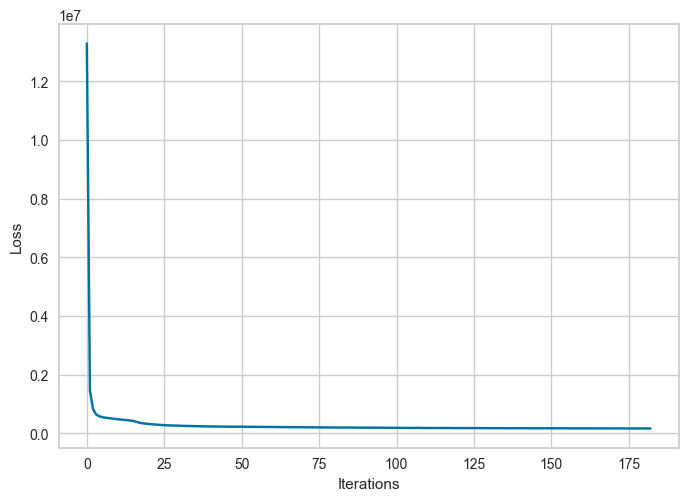
\includegraphics[width=\textwidth]{../Figures/mlp/mlp1.png}
        \caption{Wide and Deep}
        \label{fig:clarityBox}
    \end{subfigure}
    \hfill
    \begin{subfigure}[b]{0.3\textwidth}
        \centering
        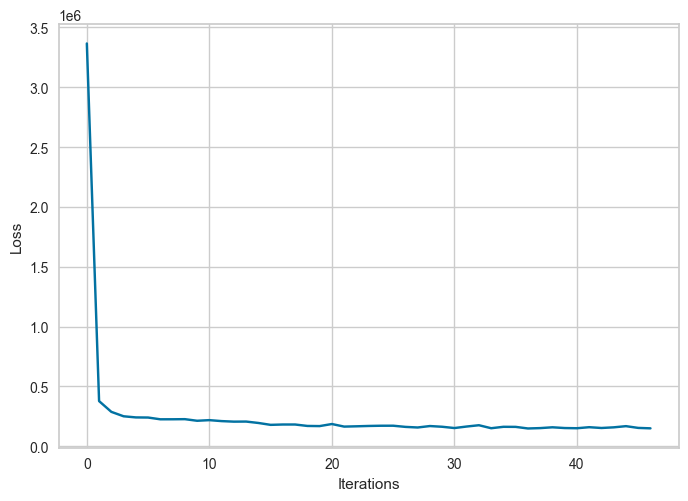
\includegraphics[width=\textwidth]{../Figures/mlp/mlp2.png}        
        \caption{Color}
        \label{fig:colorBox}
    \end{subfigure}
    \hfill
    \begin{subfigure}[b]{0.3\textwidth}
        \centering
        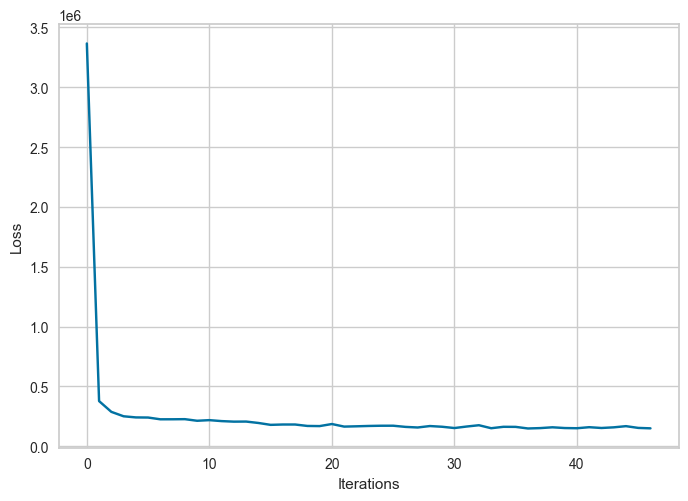
\includegraphics[width=\textwidth]{../Figures/mlp/mlp3.png}
        \caption{Cut}
        \label{fig:cutBox}
    \end{subfigure}
       \caption{Loss Curves}
       \label{fig:boxPlots}
\end{figure}
Note in this case that our Narrow and Deep network has the least neurons by far, so it is the 
preffered network—it also trained the fastest by far. 


\subsubsection*{Question 6.2}
The peformance is significantly better than the linear regression, although the time to train for even a singular 
model is almost as long as the entire grid search for linear or Ridge regression. Note that the relationship 
between our features and  \texttt{price} is probably not linear, so it is also difficult to model it with 
a simple linear regression. Meanwhile, a multilayer perceptron with multiple layers is able to construct much more 
complex non-linear functions due to the multiple layers with weights and biases. 
\subsubsection*{Question 6.3}
We did not use an activation function for the output from the last fully connected layer. Initially, we were planning on 
simply taking the output from the fully connected layer as we were just interested in the raw numebrs predicted by 
the model; however, we realized that it is an obvious assumption that the price must always be positive and as such
we decided to try RELU. However, it imperically performed worse, so we simply did not use an activation function. 
\subsubsection*{Question 6.4}
If the depth of the network is very high, the obvious risk is of course overfitting. This is simply because we are
increasing the number of neurons, so the network becomes more likely to memorize the training data. At this point,
the model would not be able to generalize as well. There is also a higher risk of vanishing or exploding gradients,
as they are carried over fro one layer onto the next layer. We also face the issue of internal covariate shift, 
where every hidden layer's input distribution has to change every time a parameter updates in the previous layer 
leading to extremely slow training that is not possible without good parameter initializations. 
\subsection*{Random Forest}
We began by noting that increasing the number of trees always increased the overall performance.
I did not increase the number of trees beyond 200 because of the time it took to run, but 
the ensembling nature of having more trees is what leads to better performance. We do not 
provide justification in ways of a graph for this but rather have our tables at the end of this 
report to justify this answer. Similarily, we will assume for the
following plot that using no function for max features is best.
\begin{figure}[H]
    \centering
        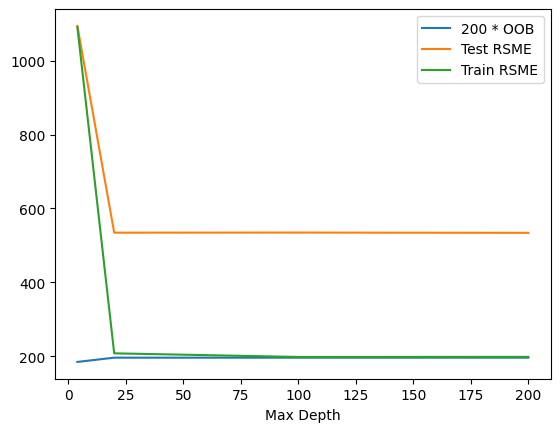
\includegraphics[width=0.4\textwidth]{../Figures/treePlot.png}
       \caption{Random Forest Loss vs Max Depth}
       \label{fig:boxPlots}
\end{figure}

\begin{table}[!ht]
    \centering
    \begin{tabular}{llll}
    \hline
        Max Depth & OOB Error & Test RSME & Train RSME \\ \hline
        4 & 0.9244489827 & 1093.68057 & 1090.131115 \\
        20 & 0.9819323954 & 534.4829574 & 208.1138089 \\
        100 & 0.9818788398 & 534.7722537 & 198.3342015 \\
        200 & 0.9818834686 & 533.9593106 & 198.5191772
    \end{tabular}
\end{table}
We thus find that our best model is that of max depth 100, no function for max features, and 
200 trees. 

\begin{table}[!ht]
    \centering
    \begin{tabular}{|l|l|l|l|l|l|}
    \hline
        Max Feature Function & Max Depth & Number of Trees & OOB & Test RSME & Train RSME \\ \hline
        Sqrt & 4 & 10 & 0.888507545 & 1159.959716 & 1152.848945 \\ \hline
        Sqrt & ~ & 50 & 0.9171313504 & 1140.563857 & 1134.275963 \\ \hline
        Sqrt & ~ & 100 & 0.9191165157 & 1129.346395 & 1123.858801 \\ \hline
        Sqrt & ~ & 200 & 0.9188510884 & 1134.089141 & 1128.10018 \\ \hline
        Sqrt & 20 & 10 & 0.9538068624 & 574.710234 & 270.643099 \\ \hline
        Sqrt & ~ & 50 & 0.9801764999 & 548.0368293 & 234.7525084 \\ \hline
        Sqrt & ~ & 100 & 0.9810110937 & 544.337696 & 229.7962548 \\ \hline
        Sqrt & ~ & 200 & 0.9813714943 & 541.9969573 & 227.829509 \\ \hline
        Sqrt & 100 & 10 & 0.952074361 & 584.8709897 & 251.5979829 \\ \hline
        Sqrt & ~ & 50 & 0.9801804006 & 548.2237846 & 209.7595994 \\ \hline
        Sqrt & ~ & 100 & 0.9809620903 & 543.0336185 & 204.1539647 \\ \hline
        Sqrt & ~ & 200 & 0.9813119671 & 540.9774691 & 201.4067505 \\ \hline
        Sqrt & 200 & 10 & 0.9524553607 & 581.9463059 & 249.9683452 \\ \hline
        Sqrt & ~ & 50 & 0.9800355171 & 549.180965 & 210.5645585 \\ \hline
        Sqrt & ~ & 100 & 0.9808838459 & 545.553042 & 204.4457473 \\ \hline
        log & ~ & 200 & 0.9813853014 & 543.6600276 & 201.2575916 \\ \hline
        log & 4 & 10 & 0.8883054168 & 1157.457366 & 1150.956749 \\ \hline
        log & ~ & 50 & 0.917231479 & 1140.118984 & 1133.194543 \\ \hline
        log & ~ & 100 & 0.919291226 & 1129.281357 & 1122.782338 \\ \hline
        log & ~ & 200 & 0.918920738 & 1134.014515 & 1127.519151 \\ \hline
        log & 20 & 10 & 0.9527329601 & 576.6097058 & 271.1668142 \\ \hline
        log & ~ & 50 & 0.9802277603 & 545.6922031 & 234.9126577 \\ \hline
        log & ~ & 100 & 0.9809636018 & 543.2411822 & 230.2138979 \\ \hline
        log & ~ & 200 & 0.981371479 & 541.1313816 & 227.5167292 \\ \hline
        log & 100 & 10 & 0.9508821205 & 582.2038386 & 251.3593473 \\ \hline
        log & ~ & 50 & 0.9801277275 & 547.6444163 & 209.9927989 \\ \hline
        log & ~ & 100 & 0.9809551574 & 542.9125848 & 203.8702072 \\ \hline
        log & ~ & 200 & 0.9813605768 & 541.0191076 & 201.3292414 \\ \hline
        log & 200 & 10 & 0.9515704197 & 578.0423422 & 250.3845501 \\ \hline
        log & ~ & 50 & 0.9801532065 & 551.3455731 & 210.0763147 \\ \hline
        log & ~ & 100 & 0.9810080433 & 544.0830238 & 203.7966355 \\ \hline
        log & ~ & 200 & 0.9813756034 & 542.2773565 & 201.1595134 \\ \hline
        none & 4 & 10 & 0.9023035324 & 1097.538401 & 1094.664785 \\ \hline
        none & ~ & 50 & 0.9241238739 & 1093.927796 & 1090.392225 \\ \hline
        none & ~ & 100 & 0.9244161312 & 1092.986609 & 1089.681183 \\ \hline
        none & ~ & 200 & 0.9244489827 & 1093.68057 & 1090.131115 \\ \hline
        none & 20 & 10 & 0.9564292592 & 557.9466554 & 242.4763037 \\ \hline
        none & ~ & 50 & 0.9812088369 & 537.8696376 & 214.0872931 \\ \hline
        none & ~ & 100 & 0.9817084472 & 535.6808118 & 210.1387262 \\ \hline
        none & ~ & 200 & 0.9819323954 & 534.4829574 & 208.1138089 \\ \hline
        none & 100 & 10 & 0.9566362724 & 558.9295058 & 235.81578 \\ \hline
        none & ~ & 50 & 0.9811235288 & 537.2029647 & 204.7660947 \\ \hline
        none & ~ & 100 & 0.9816142316 & 535.4227102 & 200.3857282 \\ \hline
        none & ~ & 200 & 0.9818788398 & 534.7722537 & 198.3342015 \\ \hline
        none & 200 & 10 & 0.956278795 & 561.0361648 & 236.9948476 \\ \hline
        none & ~ & 50 & 0.9811670519 & 540.1592345 & 205.2858802 \\ \hline
        none & ~ & 100 & 0.9816291442 & 535.0693099 & 200.8452532 \\ \hline
        none & ~ & 200 & 0.9818834686 & 533.9593106 & 198.5191772 \\ \hline
    \end{tabular}
\end{table}

\subsubsection*{Question 7.1}
Maximum number of features has a regulariation effect on the model. This is simply because we are considering less 
features, and disregarding the features that aren't as useful. As such, we have a simpler model and thus 
setting this maximum number of features for the tree to split on allows for regularization. However, eliminating
too many featuers could be harmful to the model as we could simply be eliminating features that are valuable.
The number of trees refers to the number of seperate tree models created that are going to be ensembled. The more models
we ensemble while
also using bootstrapping allows for more regualrization. However, at the same time, we must balance having enough data 
for the individual trees to actually train on. Lastly, the depth of each tree obviously has a regularization effect 
on the model, as we are effectively reducing the complexity and "number of neurons" of the model. We can also try 
to change the depth by adjusting the minimum number of samples needed in order to split into multiple leaves. 

\subsubsection*{Question 7.2}
Random forests are essentially combining small piecewise linear decision boundaries 
at each of its nodes into a larger non-linear structure. Thus, our final decision 
boundary is somewhat more complex, and can in fact be non-linear. Logically, we see
the decision tree itself can overfit any dataset y setting harsher and harsher if-statements,
meaning it can perfectly model/overfit any training set. 
\subsubsection*{Question 7.3}

\begin{figure}[H]
    \centering
        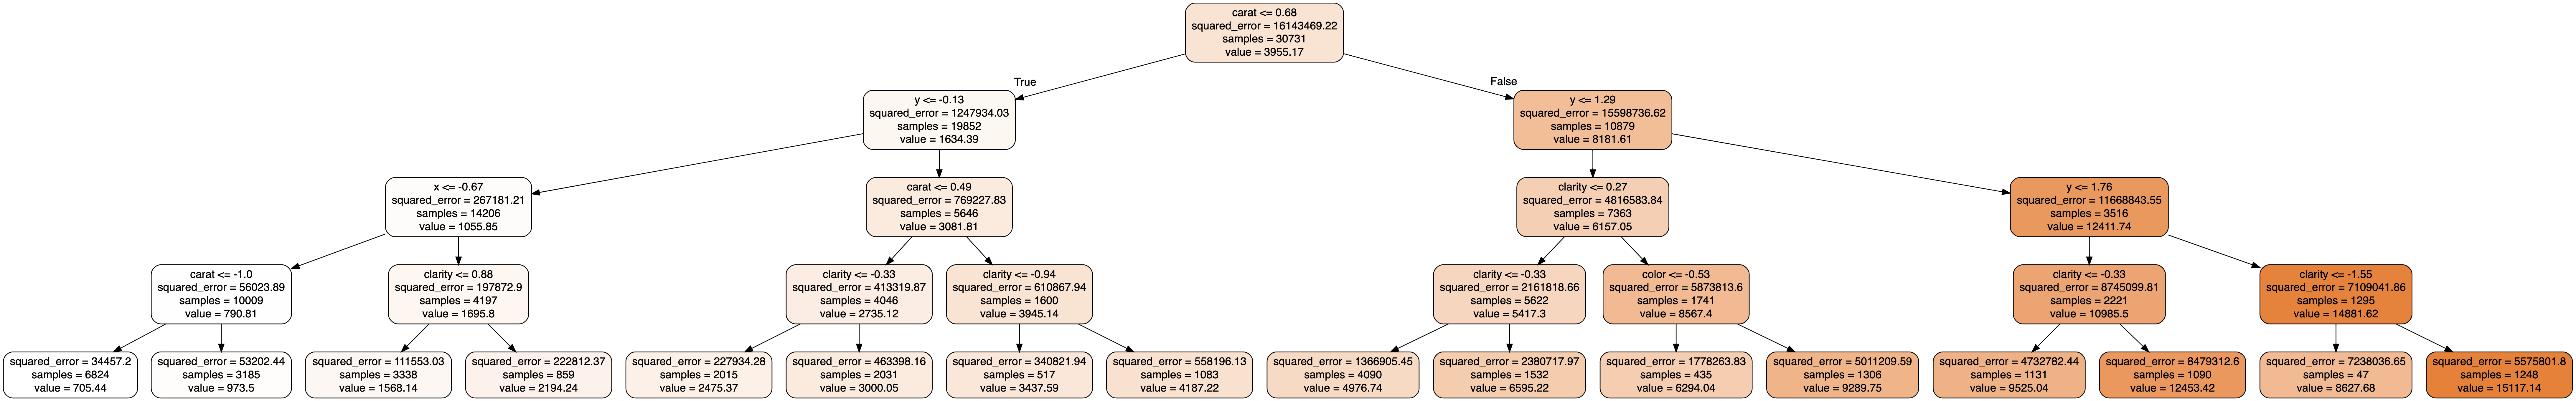
\includegraphics[width=0.8\textwidth]{../Figures/tree.png}
    \hfill
       \caption{Random 4 depth Tree from Random Forest}
       \label{fig:boxPlots}
\end{figure}

We see that the feature selected for branching at the root node is \texttt{carat} as 
expected. We noted earlier that \texttt{carat} was the most important feature, as it 
corresponds to the literal weight and size of the diamond. It also has the highest mutual 
information with \texttt{price} of all the features. It does agree with our earlier 
findings somewhat. We see that \texttt{clarity} and \texttt{color} become the most common
classifier. This generally makes sense from a human standpoint as it suggests that 
the model is getting a general ballpark of how much the diamond is worth from its weight 
and then proceding to use the finer features to price the diamond. The only exception 
is the apperance of the \texttt{x} node, by note that this too is closely correlated with 
\texttt{carat}. The reason we do not see more is because the infromation of \texttt{x} is
mostly encompassed within \texttt{carat}, as we simply care about size of the diamond. 


\subsubsection*{Question 7.4}
To explain OOB error, let us first examine how a Random Forest algorithm with
bootstrapping works. If we bootstrap, we sample the training data, and then use 
this small sample of the training data in order to train a single decision tree model.
We can then ensemble many such trees, all trained with different samples of the original
data. OOB error is calculated on the training set, where we calculate the average error 
of the trees' predictions on data that was not included in its bootstrap sample. \\\\
$R^2$ score is normally used as the coefficient of determination—that is—the proportion
of the variation in the labels that can be predicted from the features. For random 
forests, we compute it as:
\[R^2 = 1- \dfrac{\text{MSE}}{\text{Var}(\text{labels})}
    \]
Note that $R^2$ for non-linear predictors like random forest can in fact be negative.



\subsection*{LightGBM, CatBoost, and Bayesian Optimization}
\subsubsection*{Question 8.1}
The hyperparameters we chose to vary were:
\begin{enumerate}
\item[1.] \texttt{Tree_Learning_Rate} drawn from a uniform distribution betweeen 0.005 and 5
\item[2.] \texttt{Treee__max_depth} drawn as an integer value between 2 and 32 includisve
\item[3.] \texttt{tree__min_split_gain} drawn betweeen 0 and 0.3 
\item[4.] \texttt{tree__n_estimators} drawn as an integer value betweeen 100 and 200 inclusive
\item[5.] \texttt{reg_alpha} drawn as an integer value between 0 and 0.1
\end{enumerate}
We of course used \texttt{n_jobs} in order to paralalize the task. We used these 
hyperparameters, as the others did not seem very useful—we included regularization 
parameters, along with parameters like learning rate and max depth that 
allow us to make sure the model is actually learning (we don't over regularize).
\subsubsection*{Question 8.2}
Our best model corresponding to the hyperparameters refferred to in the previous question 
used (Note the order will be the same as above):
\begin{enumerate}
\item[1.] \texttt{Tree_Learning_Rate} is 0.356790985277557
\item[2.] \texttt{Tree__max_depth} is 3
\item[3.] \texttt{tree__min_split_gain} is  0.11439104645067763
\item[4.] \texttt{tree__n_estimators} is 200
\item[5.] \texttt{reg_alpha} is 0.0723842703480234
\end{enumerate}
Note it had RMSE 592.498771288194

\subsubsection*{Question 8.3}
Increasing \texttt{tree__n_estimators} is very important for better performance as it 
allows us to essentialyl ensemble more models. The more models we have voting, the higher 
our accuracy will be (provided each is given a reasonable amount of data to train). 
Increasing \texttt{Tree__max_depth} makes our model more complex and more able to model 
more non-linear loss curves; decreasing it on the other hand acts as a regularization effect as we 
are forcefully decreasing the complexity of the model by limiting it to only a certain number of 
splits. The \texttt{tree__min_split_gain} refers to the minimum loss reduction that we need to 
split a node—higher values create a sort of regularization effect as we don't allow the model to 
completely reduce the training error. Learning rate is a very standard parameters, allowing us to modify 
the SGD learning rate of the algorithm. A learning rate too low will cause us to get stuck in local 
minima while one that is too high may shoot past the solution. Choosing a good value for learning rate is 
important for converging to the solution fast. 
\pagebreak
\begin{center}
    \begin{minipage}{10cm}
    	\begin{center}
    	\textbf{\large Project 4 Twitter Data}\\[0.1cm]
        \textbf{Inesh Chakrabarti, Lawrence Liu, Nathan Wei}\\[0.1cm]
    	\end{center}
    \end{minipage}\hfill
\end{center}
\rule{17cm}{0.1mm}




%%%%%%%%%%%%%%%%%%%%%%%%%%%%%%%%%%%%%%%%%%%%%%%%%%%%%%%%%%%%%%%%%%%%%%%%%%%%%%%%
%%%%%%%%%%%%%%%%%%%%%%%%%%%%%%%%%%%%%%%%%%%%%%%%%%%%%%%%%%%%%%%%%%%%%%%%%%%%%%%%




\end{document}

